\part{Induction machine}
\title[Induction machine]{Induction machine}  
\date{}  
\frame{\titlepage} 

%%%%%%%%%%%%%%%%%%%%%%%%%%%%%%%%%%%%%%%%%%%%%%%%%%%%%%%%%%%%%
%% Basic induction machine (IM) representation %%
%%%%%%%%%%%%%%%%%%%%%%%%%%%%%%%%%%%%%%%%%%%%%%%%%%%%%%%%%%%%%
\begin{frame}
	\frametitle{Basic induction machine (IM) representation}
    \begin{columns}
		\begin{column}{0.55\textwidth}
	       \begin{itemize}
            \item Three-phase stator + three-phase rotor: ``rotating three-phase transformer''\newline (plus air gap)
            \item Rotor angular speed: $\omega_\mathrm{r}$
            \item Rotor angular displacement: $\varepsilon_\mathrm{r}$
            \item Index ``s'' for stator, ``r'' for rotor quantities
           \end{itemize}
           \begin{varblock}{Fundamental wave model}
              While the previous chapter has revealed that the magnetic flux distribution in the air gap is subject to plentiful harmonics, the following model limits itself to the fundamental wave.
           \end{varblock}
        \end{column}
        \begin{column}{0.45\textwidth}
            \begin{figure}
                \centering
                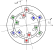
\includegraphics[width=0.85\textwidth]{fig/lec06/Simple_three_phase_induction_machine_lumped_coils.pdf}
                \caption{Elementary three-phase induction machine (IM) lumped-coil representation ($p=1$ pole pair)}
                \label{fig:Simple_three_phase_induction_machine_lumped_coils}
            \end{figure}
        \end{column}
    \end{columns}
\end{frame}

%%%%%%%%%%%%%%%%%%%%%%%%%%%%%%%%%%%%%%%%%%%%%%%%%%%%%%%%%%%%%
%% Dynamical IM model %%
%%%%%%%%%%%%%%%%%%%%%%%%%%%%%%%%%%%%%%%%%%%%%%%%%%%%%%%%%%%%%
\begin{frame}
	\frametitle{Dynamical IM model}
    Based on Faraday's and Ohm's laws, we can write the following equations for the stator 
    \begin{equation}
            \bm{u}_\mathrm{s}(t) = \bm{R}_\mathrm{s}\bm{i}_\mathrm{s}(t)+\frac{\mathrm{d}}{\mathrm{d}t}\bm{\psi}_\mathrm{s}(t) \quad \Leftrightarrow \quad \begin{bmatrix}
                u_{\mathrm{s,a}}(t)\\
                u_{\mathrm{s,b}}(t)\\
                u_{\mathrm{s,c}}(t)\\
            \end{bmatrix} = \begin{bmatrix}
                R_\mathrm{s} & 0 & 0\\
                0 & R_\mathrm{s} & 0\\
                0 & 0 & R_\mathrm{s}\\
            \end{bmatrix} \begin{bmatrix}
                i_{\mathrm{s,a}}(t)\\
                i_{\mathrm{s,b}}(t)\\
                i_{\mathrm{s,c}}(t)\\
            \end{bmatrix} + \frac{\mathrm{d}}{\mathrm{d}t} \begin{bmatrix}
                \psi_{\mathrm{s,a}}(t)\\
                \psi_{\mathrm{s,b}}(t)\\
                \psi_{\mathrm{s,c}}(t)\\
            \end{bmatrix}
    \end{equation}
    and rotor
    \begin{equation}
            \bm{u}_\mathrm{r}(t) = \bm{R}_\mathrm{r}\bm{i}_\mathrm{r}(t)+\frac{\mathrm{d}}{\mathrm{d}t}\bm{\psi}_\mathrm{r}(t) \quad \Leftrightarrow \quad \begin{bmatrix}
                u_{\mathrm{r,a}}(t)\\
                u_{\mathrm{r,b}}(t)\\
                u_{\mathrm{r,c}}(t)\\
            \end{bmatrix} = \begin{bmatrix}
                R_\mathrm{r} & 0 & 0\\
                0 & R_\mathrm{r} & 0\\
                0 & 0 & R_\mathrm{r}\\
            \end{bmatrix} \begin{bmatrix}
                i_{\mathrm{r,a}}(t)\\
                i_{\mathrm{r,b}}(t)\\
                i_{\mathrm{r,c}}(t)\\
            \end{bmatrix} + \frac{\mathrm{d}}{\mathrm{d}t} \begin{bmatrix}
                \psi_{\mathrm{r,a}}(t)\\
                \psi_{\mathrm{r,b}}(t)\\
                \psi_{\mathrm{r,c}}(t)\\
            \end{bmatrix}
    \end{equation}
which are generally applicable as only identical resistances per phase on the stator and rotor are assumed.
\end{frame}

%%%%%%%%%%%%%%%%%%%%%%%%%%%%%%%%%%%%%%%%%%%%%%%%%%%%%%%%%%%%%
%% Flux linakge model %%
%%%%%%%%%%%%%%%%%%%%%%%%%%%%%%%%%%%%%%%%%%%%%%%%%%%%%%%%%%%%%
\begin{frame}
	\frametitle{Flux linkage model}
    \begin{columns}
		\begin{column}{0.55\textwidth}
            In contrast to the simple three-phase transformer model \eqref{eq:Three_phase_transformer_flux_linkage}, the flux linkage model of the IM is more complex: 
	       \begin{itemize}
            \item Due to the spatial 120$^\circ$ phase shift between the windings of the stator and rotor, the abc phases are all mutually coupled.
            \item The flux paths and physical dimensions of the stator and rotor are not identical, i.e., the rotor and stator inductances are different (even if the winding turns $N_\mathrm{s}$ and $N_\mathrm{r}$ are identical).
            \item The coupling between the stator and rotor is rotor position-dependent (not explicitly shown on the right due to space limitations). 
           \end{itemize}
        \end{column}
        \begin{column}{0.45\textwidth}
            \begin{figure}
                \centering
                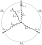
\includegraphics[width=0.75\textwidth]{fig/lec06/Inductive_coupling_stator_rotor.pdf}
                \caption{Simplified representation of the inductive coupling between the stator/rotor phases}
                \label{fig:Simple_three_phase_induction_machine_lumped_coils}
            \end{figure}
        \end{column}
    \end{columns}
\end{frame}

%%%%%%%%%%%%%%%%%%%%%%%%%%%%%%%%%%%%%%%%%%%%%%%%%%%%%%%%%%%%%
%% Flux linakge model %%
%%%%%%%%%%%%%%%%%%%%%%%%%%%%%%%%%%%%%%%%%%%%%%%%%%%%%%%%%%%%%
\begin{frame}
	\frametitle{Flux linkage model}
    Based on the previous considerations, the flux linkages are given by
    \begin{equation}
        \renewcommand*{\arraystretch}{1.15}
        \begin{split}
            \bm{\psi}_\mathrm{s}(t) &=\begin{bmatrix}
                L_\mathrm{s} & -\frac{M_\mathrm{s}}{2} & -\frac{M_\mathrm{s}}{2}\\
                -\frac{M_\mathrm{s}}{2} & L_\mathrm{s} & -\frac{M_\mathrm{s}}{2}\\
                -\frac{M_\mathrm{s}}{2} & -\frac{M_\mathrm{s}}{2} & L_\mathrm{s}
            \end{bmatrix} \bm{i}_\mathrm{s}(t) +  L_{\mathrm{r,m}}\frac{N_\mathrm{s}}{N_\mathrm{r}} \bm{\mathcal{R}}_\mathrm{abc}(\varepsilon_\mathrm{r,el})\bm{i}_\mathrm{r}(t)\\
            \bm{\psi}_\mathrm{r}(t) &= \begin{bmatrix}
                L_\mathrm{r} & -\frac{M_\mathrm{r}}{2} & -\frac{M_\mathrm{r}}{2}\\
                -\frac{M_\mathrm{r}}{2} & L_\mathrm{r} & -\frac{M_\mathrm{r}}{2}\\
                -\frac{M_\mathrm{r}}{2} & -\frac{M_\mathrm{r}}{2} & L_\mathrm{r}
            \end{bmatrix} \bm{i}_\mathrm{r}(t) +  L_{\mathrm{s,m}}\frac{N_\mathrm{r}}{N_\mathrm{s}} \bm{\mathcal{R}}_\mathrm{abc}(\varepsilon_\mathrm{r,el})\bm{i}_\mathrm{s}(t) 
        \end{split}
    \end{equation}
    with $\varepsilon_\mathrm{r,el}=p\varepsilon_\mathrm{r}$ and the transformation matrix
    \begin{equation}
        \renewcommand*{\arraystretch}{1.15}
        \bm{\mathcal{R}}_\mathrm{abc}(\varepsilon_\mathrm{r,el}) =\begin{bmatrix}
           \cos(\varepsilon_\mathrm{r,el})  & \cos(\varepsilon_\mathrm{r,el} - \frac{2\pi}{3}) & \cos(\varepsilon_\mathrm{r,el} + \frac{2\pi}{3})\\
            \cos(\varepsilon_\mathrm{r,el} + \frac{2\pi}{3}) & \cos(\varepsilon_\mathrm{r,el}) & \cos(\varepsilon_\mathrm{r,el} - \frac{2\pi}{3})\\
            \cos(\varepsilon_\mathrm{r,el} - \frac{2\pi}{3}) & \cos(\varepsilon_\mathrm{r,el} + \frac{2\pi}{3}) & \cos(\varepsilon_\mathrm{r,el})
        \end{bmatrix}.
    \end{equation}
\end{frame}

%%%%%%%%%%%%%%%%%%%%%%%%%%%%%%%%%%%%%%%%%%%%%%%%%%%%%%%%%%%%%
%% \frametitle{Inductance matrices} %%
%%%%%%%%%%%%%%%%%%%%%%%%%%%%%%%%%%%%%%%%%%%%%%%%%%%%%%%%%%%%%
\begin{frame}
	\frametitle{Inductance matrices}
    The inductance matrices
    $$\renewcommand*{\arraystretch}{1.15} 
    L_\mathrm{s,abc} = \begin{bmatrix}
        L_\mathrm{s} & -\frac{M_\mathrm{s}}{2} & -\frac{M_\mathrm{s}}{2}\\
        -\frac{M_\mathrm{s}}{2} & L_\mathrm{s} & -\frac{M_\mathrm{s}}{2}\\
        -\frac{M_\mathrm{s}}{2} & -\frac{M_\mathrm{s}}{2} & L_\mathrm{s}
    \end{bmatrix}, \qquad  L_\mathrm{r,abc} = \begin{bmatrix}
        L_\mathrm{r} & -\frac{M_\mathrm{r}}{2} & -\frac{M_\mathrm{r}}{2}\\
        -\frac{M_\mathrm{r}}{2} & L_\mathrm{r} & -\frac{M_\mathrm{r}}{2}\\
        -\frac{M_\mathrm{r}}{2} & -\frac{M_\mathrm{r}}{2} & L_\mathrm{r}
    \end{bmatrix}$$
    are based on the following considerations. 
\end{frame}